\documentclass[11pt]{report}

\usepackage[portuguese]{babel}
\usepackage[utf8]{inputenc}
\usepackage{graphicx}
\usepackage{hyperref}
\usepackage{indentfirst}
\usepackage{kantlipsum}
\usepackage{float}
\usepackage{listings}
\usepackage{mathtools}
\usepackage{amsmath}
\usepackage{url}
\usepackage[margin=0.8in]{geometry}
\usepackage{biblatex}
\usepackage{multirow}
\usepackage{fancyhdr}
\usepackage[table,xcdraw]{xcolor}
\bibliography{biblio.bib}

\lstset{language=Prolog}

\hypersetup{
    colorlinks=true,
    linkcolor=black,
    citecolor=black,
    filecolor=black,
    urlcolor=black
}

\newlength{\normalparindent}
\setlength{\normalparindent}{\parindent}
\setlength{\parindent}{\normalparindent}

\newcommand{\blank}[1]{\hspace*{#1}}

\renewcommand{\headrulewidth}{0pt}

\pagestyle{fancy}
\fancyhf{}
\rhead{
\includegraphics [scale=0.5]{uproject_new_2.png}}
\rfoot{\thepage}

\begin{document}

\thispagestyle{empty}

\begin{center}
	
	
\includegraphics [scale=0.5]{uplogo500.png}
	\linebreak \linebreak \linebreak \linebreak \linebreak
	\linebreak \linebreak \linebreak \linebreak \linebreak
	\begin{Huge}
		\textbf{U.Project Website} \linebreak \linebreak
	\end{Huge}
	\begin{Large}
		\textbf{Relatório de Estágio} \linebreak \linebreak
	\end{Large}
	\linebreak
	\linebreak
	\linebreak
	\linebreak
	\linebreak
	\linebreak
	Orientadores:
	\linebreak
	\linebreak
	Bruno Fernando Reis Ribeiro Silva - \href{mailto: brunosilva@uproject.pt}{\texttt{brunosilva@uproject.pt}}
	\linebreak
	Márcio Filipe Vilela Fontes - \href{mailto: marciofontes@uproject.pt}{\texttt{marciofontes@uproject.pt}}
	\linebreak
	\linebreak
	\linebreak
	\linebreak
	UPTEC - Parque de Ciência e Tecnologia da Universidade do Porto
	\linebreak
	Rua Alfredo Allen, nº455/461, 4200-135 - Porto, Portugal
	\linebreak
	\linebreak
	\linebreak
	\linebreak
	23 de Setembro de 2015
\end{center}

\newpage

\pagenumbering{roman}


\chapter*{Agradecimentos}
\addcontentsline{toc}{chapter}{Agradecimentos}
Este trabalho não teria sido possível sem a colaboração e a boa vontade daqueles irei citar. A todos os meus sinceros agradecimentos. 

À professora Maria José Costa, orientadora deste estágio, um agradecimento muito especial por todo o apoio e pela oportunidade que me deu ao incluir-me nesta empresa. Agradeço-lhe, ainda, por ter encarnado realmente o papel, que julgo ser aquele que se espera de um orientador, isto é, por se preocupar connosco mesmo sem nós lhe pedirmos nada.

Ao Bruno Silva, fundador da empresa U.Project, que nos orientava do ponto de vista da organização das nossas atividades, pela disponibilidade, interesse e empenho com que nos recebeu.

 Ao Márcio Fontes,Co-Fundador da U.Project, pela paciência e dedicação que teve na fase inicial em nos ensinar linguagens de programação para a Internet, entre outras ferramentas. E também pelo apoio dado durante esta segunda fase de estágio nos modelos UML e também nas estruturas dos relatórios.
 
Ao professor Carlos Neves, que nos ajudou nas aulas de Técnicas de Programação a ter um melhor raciocínio e lógica em termos de programação, e pela exigência nas tarefas que proporcionava.

Agradeço também ao professor Avelino Pereira pela sua constante disponibilidade em nos responder a qualquer dúvida que surgia durante a realização das atividades que nos propunham, quer fossem da sua disciplina, matemática ou qualquer outra disciplina. Sem a sua preciosa ajuda, eu provavelmente não estava onde estou agora com classificações deste nível.

\newpage

\chapter*{Sumário}
\addcontentsline{toc}{chapter}{Sumário}
Neste relatório, serão mencionados todos os pontos relativos ao grupo ß no desenvolvimento do website para a empresa U.Project, tais como o protótipo de design Mobile e Desktop, descrição da preparação dos passos a executar, os seus objetivos e as suas funcionalidades.
 
Será também abordado o tema da empresa em si, onde explicaremos o seu funcionamento, os seus objetivos, historial, áreas de negócio, logótipo e localização.

Depois da empresa, será descrito o projeto que está agora em andamento, ou seja, os seus objetivos e funcionalidades, descrevendo também as ferramentas utilizadas, calendarização e fases de desenvolvimento.

 No final deste relatório está também uma opinião minha sobre os maiores contratempos que ocorreram durante a realização deste projeto.
\newpage

\chapter*{Abstract}
\addcontentsline{toc}{chapter}{Abstract}
In this report, all the points concerning U.Project and the creation of their website will be mentioned, such as the development stages, description from the development phases, objectives and features. 


The company itself will be described too. Its operations, objectives, history, business areas, logo and location will be shown.


After the company, the project that is now under way will also be explained, its goals and features will be described, just as the tools used, timing and stages of development. 


At the end of this report there is also a personal opinion from me about the setbacks that we suffered during the development of this project.
\tableofcontents

\newpage

\pagenumbering{arabic}

\newpage

\chapter{Introdução}

\section{Descrição}
Nesta semana inicial da fase final de estágio foi-nos pedido que fosse realizada uma proposta de website responsivo, de fácil utilização e manutenção para a U.Project.

Com o objetivo de facilitar a organização do trabalho foram criadas 3 equipas, composta por 2 elementos cada.

Na minha equipa, composta por mim e pelo Gilberto Pereira, ficamos encarregues de criar os protótipos de design para o website, com versões Desktop e Mobile.

Esta parte do trabalho foi organizada com a ajuda do Photoshop CS6, que cumpriu perfeitamente o seu papel no que toca a ferramentas de desenho.

Nesta última semana, fiquei também encarregue de ajudar a finalizar o modelo UML e a começar o modelo de base de dados juntamente com o Pedro Barbosa.



\section{Objetivo}
Este relatório tem como objetivo descrever o trabalho realizado pelo grupo ß no website para a U.Project, durante a fase final deste estágio.

\section{Estrutura do Relatório}
O relatório está dividido pelos seguintes tópicos:
\begin{itemize}
    \item Introdução - onde é exposta a descrição do relatório;
    \item A Empresa - onde se fala sobre a empresa: caracterização, objetivos, historial, estrutura hierárquica, áreas de negócio, logótipo e localização;
    \item O Projeto - onde se fala acerca do projeto: descrição, objetivos, funcionalidades, ferramentas a utilizar, atividades a desenvolver, calendarização e fases de implementação;
    \item Considerações Finais - onde está a minha opinião acerca do projeto.
\end{itemize}
\chapter{A Empresa}

\section{Caraterização da Empresa}
A U.Project é uma organização com a missão de potenciar e impulsionar o empreendedorismo jovem. Para isso, atua em duas frentes vitais para permitir às Startups criar e desenvolver as suas ideias que, de outro modo, seriam praticamente impossíveis de serem concretizadas devido aos custos e desafios envolvidos no processo.

Em primeiro lugar pretende, através da U.Project Startup Network, oferecer diversos modelos de contrato adaptados a cada Empresa de modo a que estas tenham acesso aos recursos e serviços necessários ao seu desenvolvimento.

Em segundo lugar acompanha e orienta, através da U.Project Academy, os alunos desde o ensino secundário, de modo a potenciar e desenvolver as suas capacidades para poderem participar no desenvolvimento de novos projetos e ideias. Através de um programa de estágio, em parceira com as respetivas escolas, os alunos têm acesso a diversas formações e atividades, além de terem a possibilidade de integrar uma equipa de desenvolvimento.

Para além de fornecer os seus serviços, a U.Project pretende também criar uma rede interna de empresas, de modo a que estas possam encontrar de uma forma fácil e rápida os serviços que necessitam, através do produto de outras pertencentes à rede, permitindo assim a realização de melhores negócios e um aumento na divulgação das mesmas.

Os associados da organização podem usufruir de diversos serviços e formações através do pagamento de uma quota. Quem achar que possui os requisitos necessários para trabalhar a tempo inteiro pode candidatar-se a membro, trabalhando diretamente para a empresa e usufruindo de um salário fixo de acordo com a posição ocupada, podendo também ser promovido pela direção a um cargo superior.

Quando um membro ultrapassar os 30 anos, pode ser premiado com o título de membro honorário, ficando isente do pagamento de quotas e passando a ter funções de aconselhamento e divulgação.

\section{Objetivos da Empresa}
A U.Project tem como objetivo promover o empreendedorismo jovem, dando apoio às Startups, para que estas se consigam desnevolver sem a necessidade de possuir vastos recursos financeiros.
Para isso a U.Project irá acompanhar os jovens desde o ensino secundário, apoiando-os e orientando-os na vida Universitária através da realização de estágios, competições e atividades.
Também irá estimular e incentivar estes alunos a desenvolverem as suas ideias e projetos, aproximando-os das Startups, fomentando assim o emprego jovem e garantindo um acompanhamento ao desenvolvimento dos seus projetos.

\section{Historial da Empresa}
A U.Project conta já com mais de um mês de atividade, durante o qual estabeleceu contactos com algumas empresas estrangeiras, como é o caso da Uppersky e da REDdy.

Também participou na criação de uma empresa de um estudante do MIET (Mestrado em Inovação e Empreendedorismo Tecnológico) que, por ter ficado satisfeito com a qualidade do serviço prestado, tem promovido a organização a outras empresas.

Além destes projetos, tem recebido diversos pedidos de consultoria por parte de diversas pessoas individuais.

A empresa é composta por oito membros, donde se destacam os seus dois co-fundadores, pela sua larga história pessoal e empreendedora, na qual se incluem diversos projetos e empresas. 

Encontra-se em curso uma campanha de recrutamento e de angariação de associados, de modo a que seja possível ter os recursos necessários à realização da sua missão.
\section{Estrutura Hierárquica}

Direção
\begin{itemize}
\item Presidente - Bruno Silva
\item Vice-Presidente - Márcio Fontes
\item Secretário - José Coutinho
\end{itemize}
Departamento de Comunicação e Imagem
\begin{itemize}
\item Catarina Reis
\item João Marques
\item Jorge Loures
\item Rita Cardoso
\item Tatiana
\end{itemize}
Conselho Científico
\begin{itemize}
\item Nuno Flores
\end{itemize}

\section{Áreas de Negócio}
A U.Project fornece recursos às Startups interessadas em começar o seu negócio no mundo Empresarial, permitindo assim uma redução significativa nos seus custos.

Um dos seus projetos consiste na criação de uma rede interna de empresas parceiras, denominada de U.Project Startup Network. Esta permite que as empresas participantes possam usufruir dos serviços de outras, facilitando assim os seus negócios e reduzindo os custos no processo.

Também atua no mundo académico, acompanhando os alunos desde o ensino secundário, orientando-os e ajudando-os a integrarem-se no mundo empresarial, fornecendo-lhes pelo caminho diversas aptidões e conhecimentos essenciais para a sua carreira escolar e profissional. 

Além disso, também são organizados diversos eventos, tais como formações, workshops e concursos, com vista a estimular as capacidades destes alunos e ajudá-los a cumprir os seus objetivos a nível pessoal e profissional.
\section{Logótipo}
\begin{center}

\includegraphics [scale=0.5]{uplogo500.png}
\label{img1}
\end{center}
\section{Localização}
\textbf{UPTEC - Parque de Ciência e Tecnologia da Universidade do Porto} 


Morada:
Rua Alfredo Allen, n.º455/461
4200-135 Porto


GPS:
+41º 10'38,89'' N, -8º 36'18,25'' O


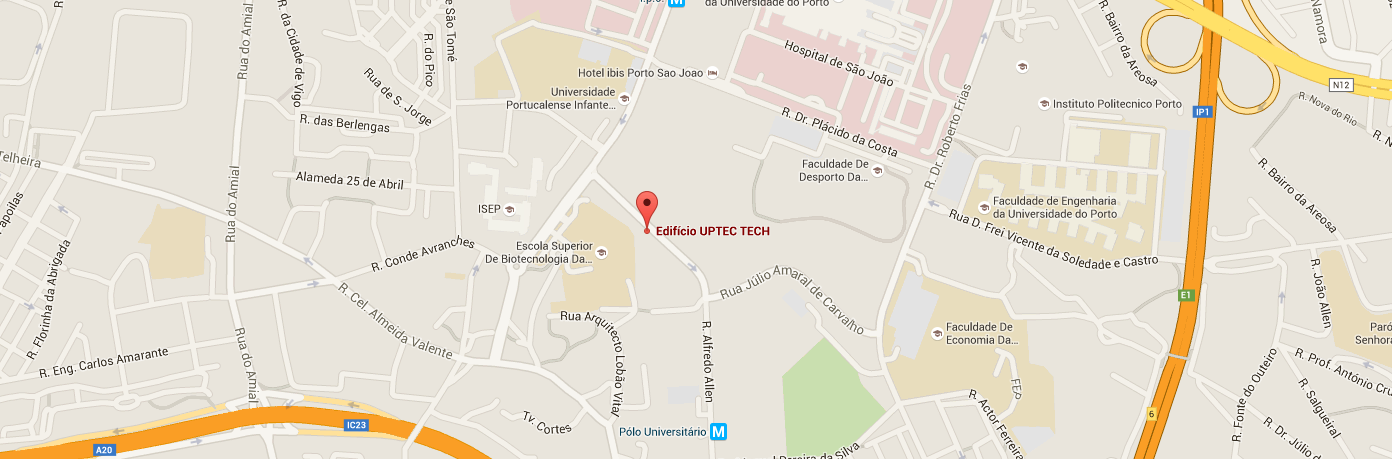
\includegraphics [scale=0.35]{location.png}
\label{img2}
\newpage

\chapter{O Projeto}
\section{Descrição}
O projeto que nos foi confiado foi o da criação de um website para a U.Project.
Este website está a ser desenvolvido de maneira a satisfazer vários objetivos distintos.
O primeiro objetivo é publicitário, pois uma das melhores maneiras de dar uma empresa a conhecer ao publico é através de um website simples, funcional, atrativo e que dê as todas as informações nesessárias tanto ao publico em geral, como a empresas ou empreendedores que queiram criar uma parceria com a U.Project.


O segundo objetivo, mas não menos importante, é o de criar uma área restrita e privada a todos os membros e associados da U.Project para que possam ter o seu grupo de trabalho dentro do próprio website com o objetivo de conseguirem gerir melhor as suas atividades e de se darem a conhecer aos outros membros atrevés de um perfil pessoal.

A direção possui também aqui uma ferramenta vital para facilitar o seu trabalho de gestão e controlo, desde os recursos humanos, até às notícias públicas e aos recursos financeiros da organização.

Espera-se que este projeto venha a contribuir para um aumento significativo da visibilidade da U.Project em Portugal e no mundo, permitindo assim alcançar os seus objetivos.
\section{Objetivos}
No Final do desenvolvimento do website, este tem que cumprir os seguintes requisitos:
\begin{itemize}
\item Estar \textit{up and running};
\item Ser um website funcional;
\item O website tem que ter página para registar utilizadores;
\item O website tem que ser capaz de fazer login e logout;
\item O website tem que ser capaz de inscrever um utilizador nas atividades que irão decorrer;
\item Um utilizador com permissões suficientes tem que ser capaz de alterar as páginas, sistema de pontos, projetos, departamentos e dados/membros da empresa a que tem acesso através de uma página de edição;
\item Um utilizador tem que conseguir pesquisar sobre o que o mesmo queira saber;
\item O website tem que ser um website dinâmico e responsivo;
\end{itemize}
\section{Funcionalidades}
\begin{itemize}
\item Formulário de Contacto;
\item Newsletter;
\item Interação com redes sociais;
\item Acesso restrito ao login;
\item Parte administrativa com capacidade de alterar qualquer página que o utilizador tenha permissão;
\item Slideshow na página inicial;
\item Página de notícias;
\item Página de eventos a decorrer e eventos futuros;
\item Interação com o Google maps;
\item Chat para comunicação entre amigos;
\item Interação com os departamentos e possibilidade de se inscrever.
\end{itemize}
\newpage
\section{Ferramentas a utilizar}

\linebreak

NOTA: Estas foram as ferramentas utilizadas pelo meu grupo.

 Não está aqui representada a totalidade das aplicações utilizadas para o desenvolvimento do Website.
\bigskip
\linebreak

\linebreak

\linebreak

\centering
\begin{minipage}{.45\linewidth}
	O Adobe Photoshop é uma aplicação de edição de imagens disponível para Microsoft Windows, Mac OS e Linux através do WINE.

	Esta é a ferramenta de edição de imagens de eleição pela maioria das pessoas por ser simples o suficiente para ser usada por novatos e ao mesmo tempo ter ferramentas complexas de grande qualidade e utilidade para satisfazer os profissionais mais exigentes.
	
	Foi utilizada para criar os protótipos das interfaces mobile e desktop do nosso website, como mostram as fotografias nos anexos.\\
\end{minipage}
\hspace{.15\linewidth}
\begin{minipage}{.20\linewidth}
  
\includegraphics[width=\linewidth]{photoshop.png}
  \caption{Logótipo do Adobe Photoshop}
  \label{img3}
\end{minipage}



\centering
\begin{minipage}{.45\linewidth}
	O Notepad++ é uma ferramenta básica de programação HTML, CSS, PhP e JS. Cumpre a mesma função que um bloco de notas com a adição de mudar a cor do texto caso seja sintaxe, atributos, etc ou mantém-lo com a cor preta caso seja conteúdo. Tem também funções como atalhos para executar o código em diferentes Browsers, gravação de Macros e capacidade de incluir Plugins para acelerar, facilitar e melhorar o trabalho do programador.
	
	Foi utilizado para editar o código Bootstrap do nosso website. \\
\end{minipage}
\hspace{.15\linewidth}
\begin{minipage}{.20\linewidth}
  
\includegraphics[width=\linewidth]{note.jpg}
  \caption{Logótipo do Notepad++}
  \label{img4}
\end{minipage}

\centering
\begin{minipage}{.45\linewidth}
	O \LaTeX\ é uma ferramenta de edição de texto constituida por um conjunto de Macros para o programa \TeX\, que é utilizado maioritariamente para fins académicos devido à sua capacidade de produzir fórmulas e símbolos matemáticos de uma forma elegante.
	
	Foi usado para produzir este relatório.\\
\end{minipage}
\hspace{.15\linewidth}
\begin{minipage}{.20\linewidth}
  
\includegraphics[width=\linewidth]{LaTeX.png}
  \caption{Logótipo do LaTeX}
  \label{img5}
\end{minipage}

\centering
\begin{minipage}{.45\linewidth}
	O GitHub é um repositório que funciona através de \textit{Web Hosting} e é utilizado para guardar e partilhar projetos de forma profissional e segura, pois permite  , por exemplo, confirmação de submissão de um novo ficheiro para o repositório, o que reduz consideravelmente o risco de aapagar-mos ou substituir-mos um arquivo acidentalmente.
	
	Foi usado para guardar e partilhar os ficheiros referentes ao Website e a todas as nossas atividades.\\
\end{minipage}
\hspace{.15\linewidth}
\begin{minipage}{.20\linewidth}
  
\includegraphics[width=\linewidth]{Git.png}
  \caption{Logótipo do Git Hub}
  \label{img6}
\end{minipage}



\newpage
\section{Atividades a desenvolver}
\addcontentsline{toc}{chapter}{Atividades a desenvolver}
Foi cancelada a parte de design do website que era destinada ao nosso grupo.

Fomos então encarregues de ajudar a finalizar o modelo UML da base de dados e  ajudar na criação do esquema relacional.


\section{Fases de Implementação}
\addcontentsline{toc}{chapter}{Fases de Implementação}

\subsection{A3 - Protótipo de interface}
	Nesta fase, utilizámos o Photoshop CS6 para criar um protótipo de interface móvel e desktop em conjunto com a equipa da base de dados, para que cumprisse todos os requisitos de funcionalidades desejadas.
	
	
\subsection{A6 - Esquema relacional}
	O esquema relacional é um modelo UML levado á prática e coloca-nos cada vez mais perto de implementar uma base de dados funcional.


\subsection{Especificação de Requisitos}

Era desejado que independentemente do estado do utilizador (registado ou não) lhe fosse possivel ter acesso ás noticias públicas escritas no \textit{News Feed} da página principal do website.
Caso o utilizador esteja registado, então teria acesso a links extra na barra principal, que lhe dão acesso ao seu perfil, opções de conta e a páginas confidenciais onde apenas utilizadores que pertencem a esse grupo conseguem aceder.
Um dos requesitos base do website é também a existência de administradores, pois apenas eles conseguem adicionar ou remover membros (aprovações de perfis ou remoção de contas) e criar os grupos para equipas de trabalho restritos para os seus parceiros.

\begin{itemize}
		
\item Só um utilizador registado tem acesso ás informações restritas.

\item Um grupo de administradores e head-admins para gerir o website, membros e equipas de desenvolvimento.

\item Estrutura de design \textit{responsive} para ecrãs de grandes e pequenas dimensões.
\end{itemize}

\chapter{Considerações Finais}

\section{Dificuldades}
Na realização deste trabalho, foram vários os problemas com que nos deparamos e que eventualmente acabaram por atrasar uma ou várias equipas e causáram-nos algumas dores de cabeça, como por exemplo a tentativa de combinar código de vários \textit{Bootstraps} num só, coisa que ao fim de dois dias de trabalho vimos que não era possivel de fazer.
Depois de desistir-mos desta ideia, decidimos eleger um só modelo de Website e trabalhar-lo, mas o problema foi escolher um modelo com que toda a gente concordasse.
Outro probelema foi por exemplo quando em cooperação com o Pedro Barbosa começamos a fazer o Modelo Relacional da base de dados. Nenhum de nós tinha feito um modelo daquela dimensão e o inicio foi bastante complicado, mas com o tempo ficou mais fácil graças ao link do LBAW que o Márcio e o Bruno nos proporcionaram.

\newpage

\begin{thebibliography}{9}
\bibitem{uproj} 
Página da U.Project
\\\texttt{http://uproject.pt/}

\bibitem{lbaw} 
LBAW

\bibitem{tex} 
Página oficial do TeX Maker
\\\texttt{https://latex-project.org/}

\bibitem{git} 
Explicação de o que é GitHub
\\\texttt{http://www.howtogeek.com/180167/htg-explains-what-is-github-and-what-do-geeks-use-it-for/}

\bibitem{notepad} 
Página oficial do Notepad++
\\\texttt{https://notepad-plus-plus.org/features/}

\bibitem{photshop} 
Explicação de o que é o Photoshop
\\\texttt{http://www.businessdictionary.com/definition/Photoshop.html}
\end{thebibliography}


\chapter{Anexos}

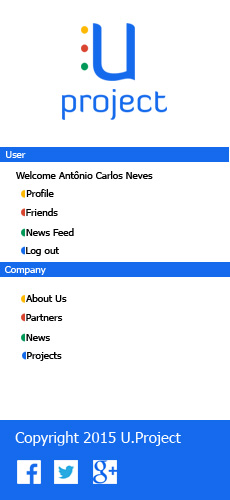
\includegraphics[\linewidth, height=15cm]{layoutmobile.jpg} 

\caption{Figura 1: Menu Mobile da Página}

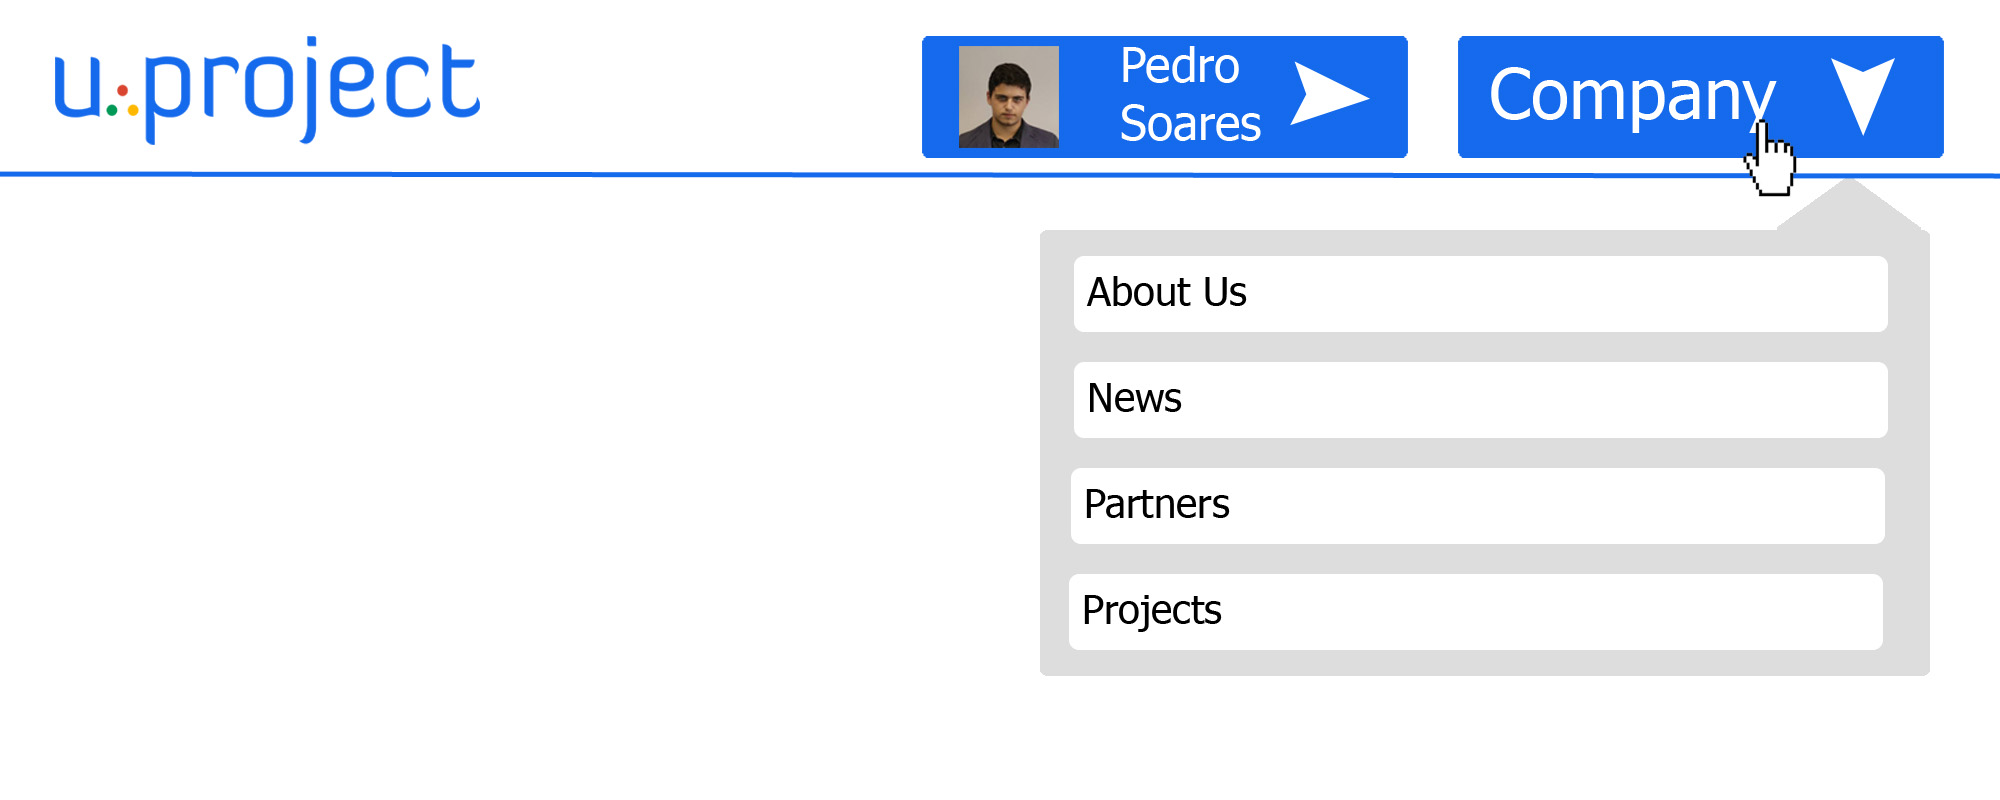
\includegraphics[\linewidth, height=7cm]{layoutpc.jpg} 

\caption{Figura 2: Menu Desktop da Página}

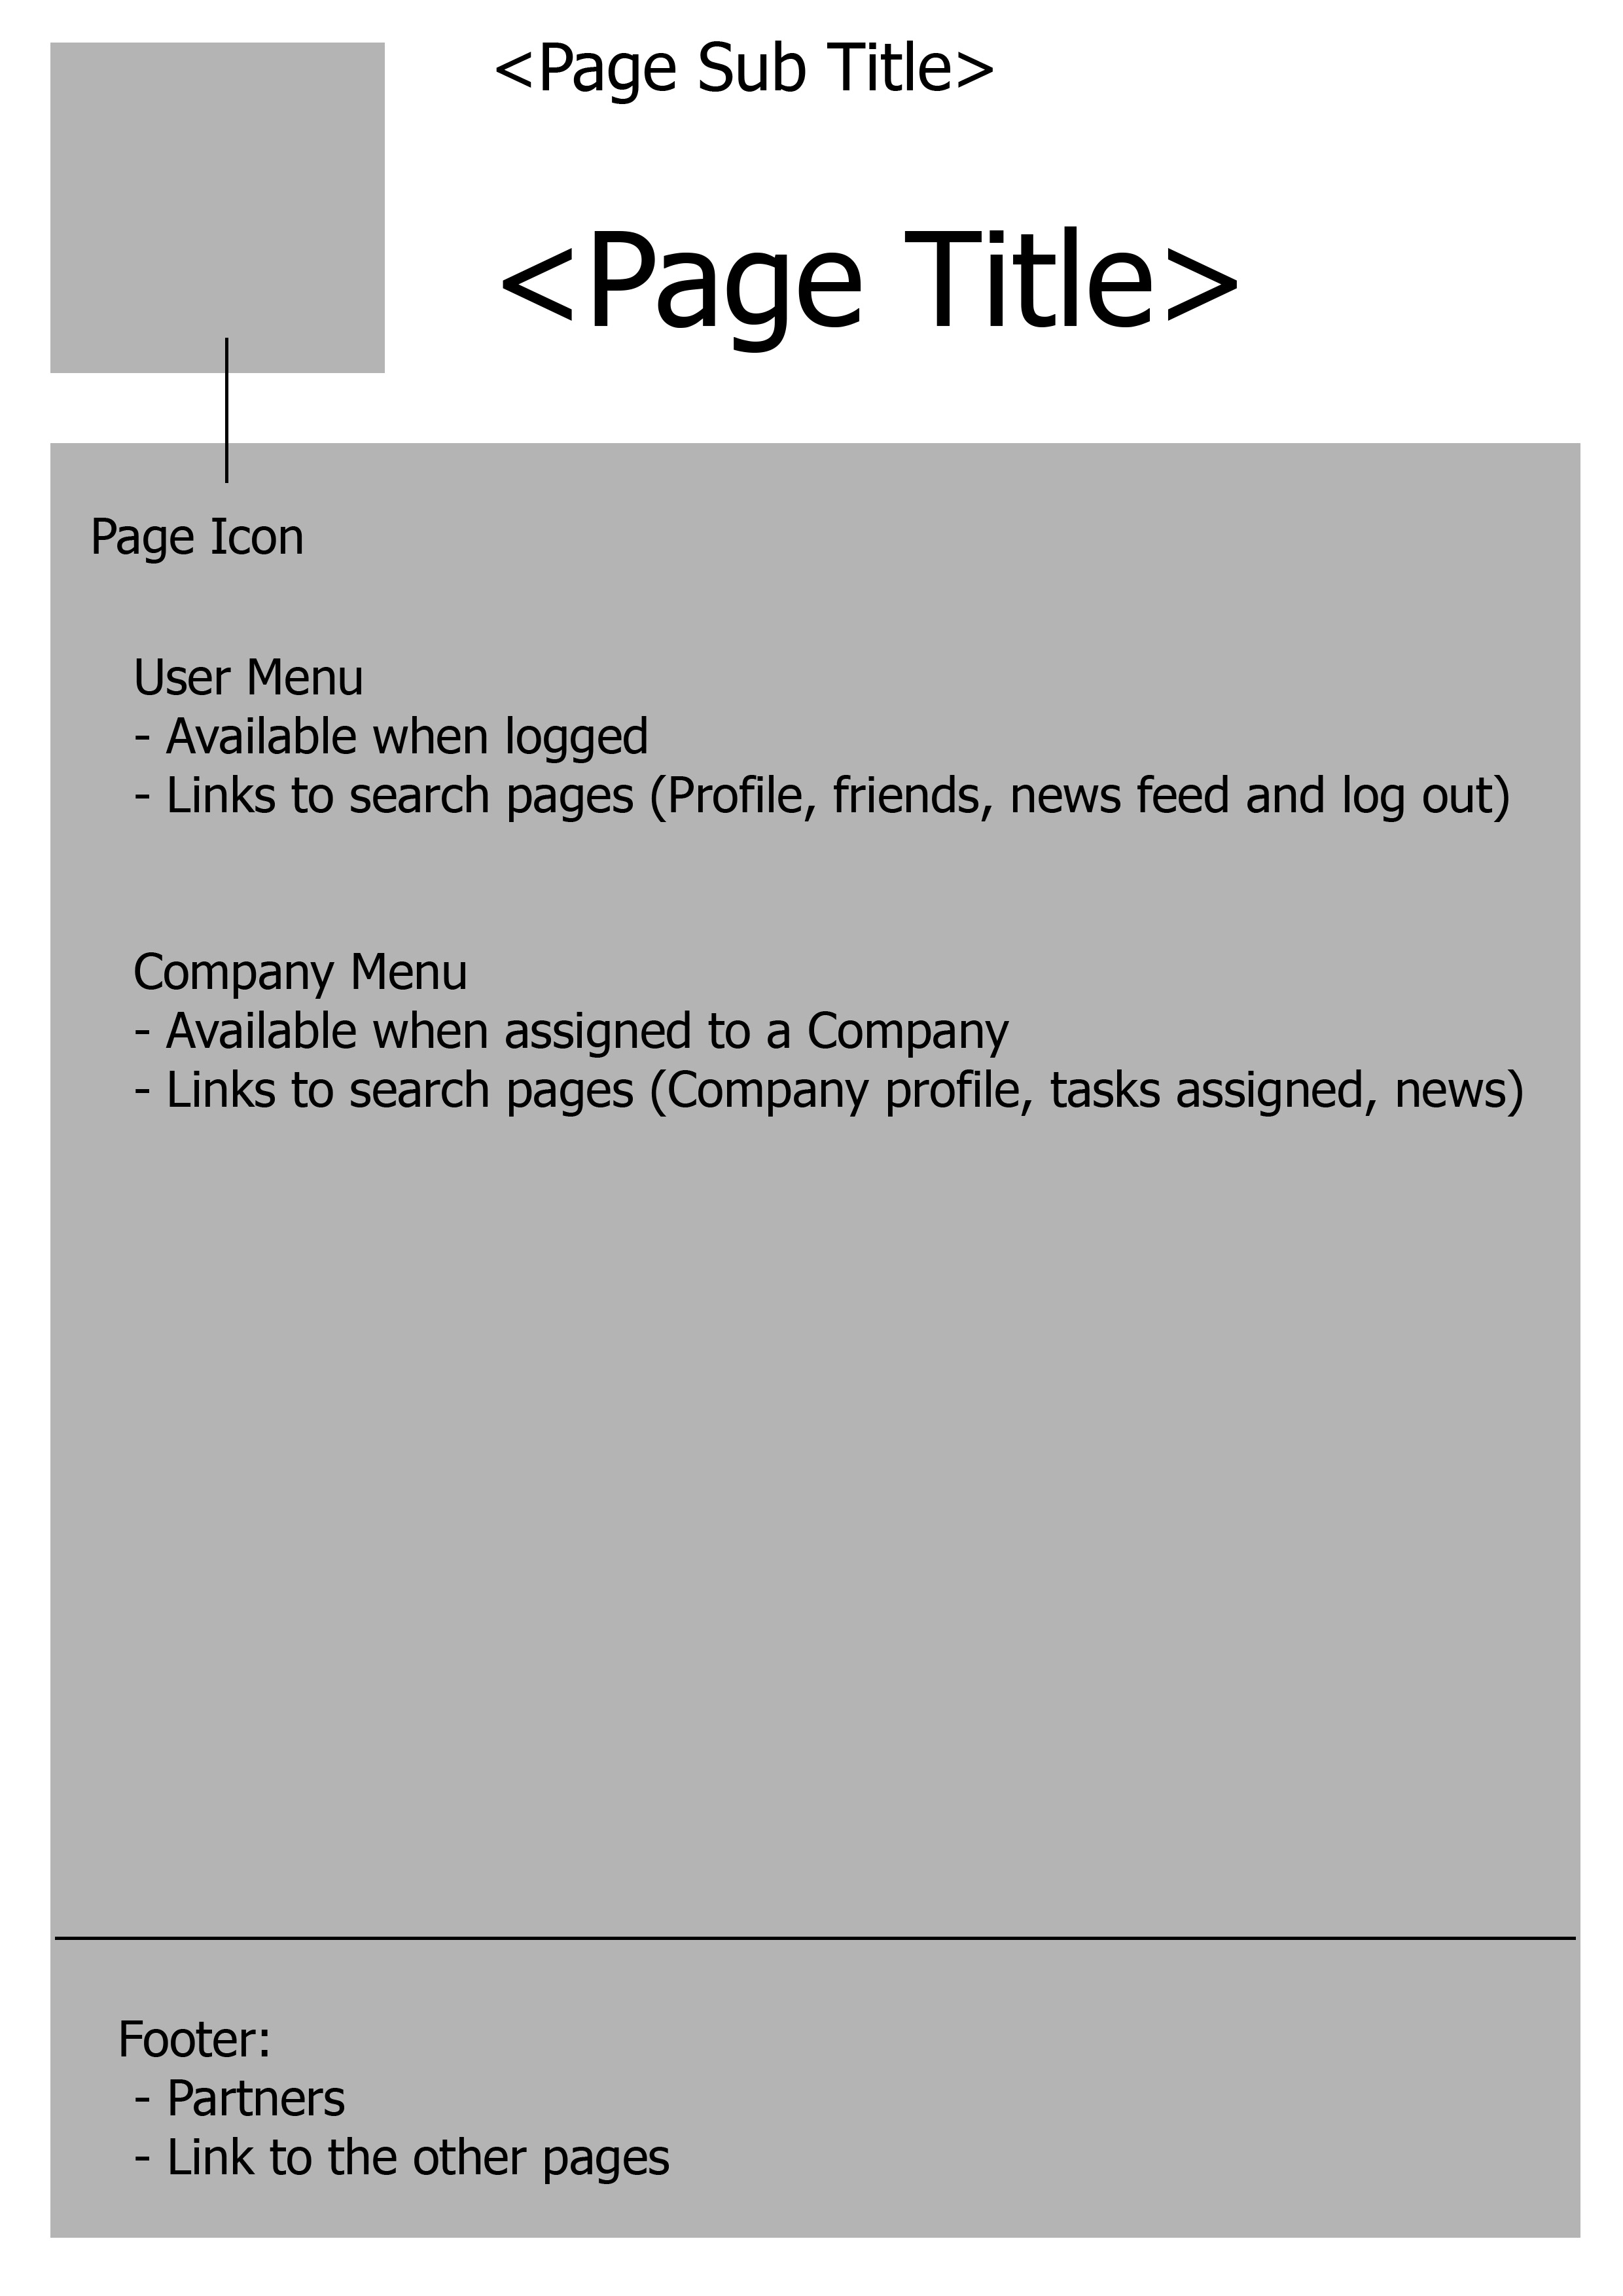
\includegraphics[\linewidth, height=15cm]{layoutpagina.jpg} 

\caption{Figura 3: Layout da Pagina}

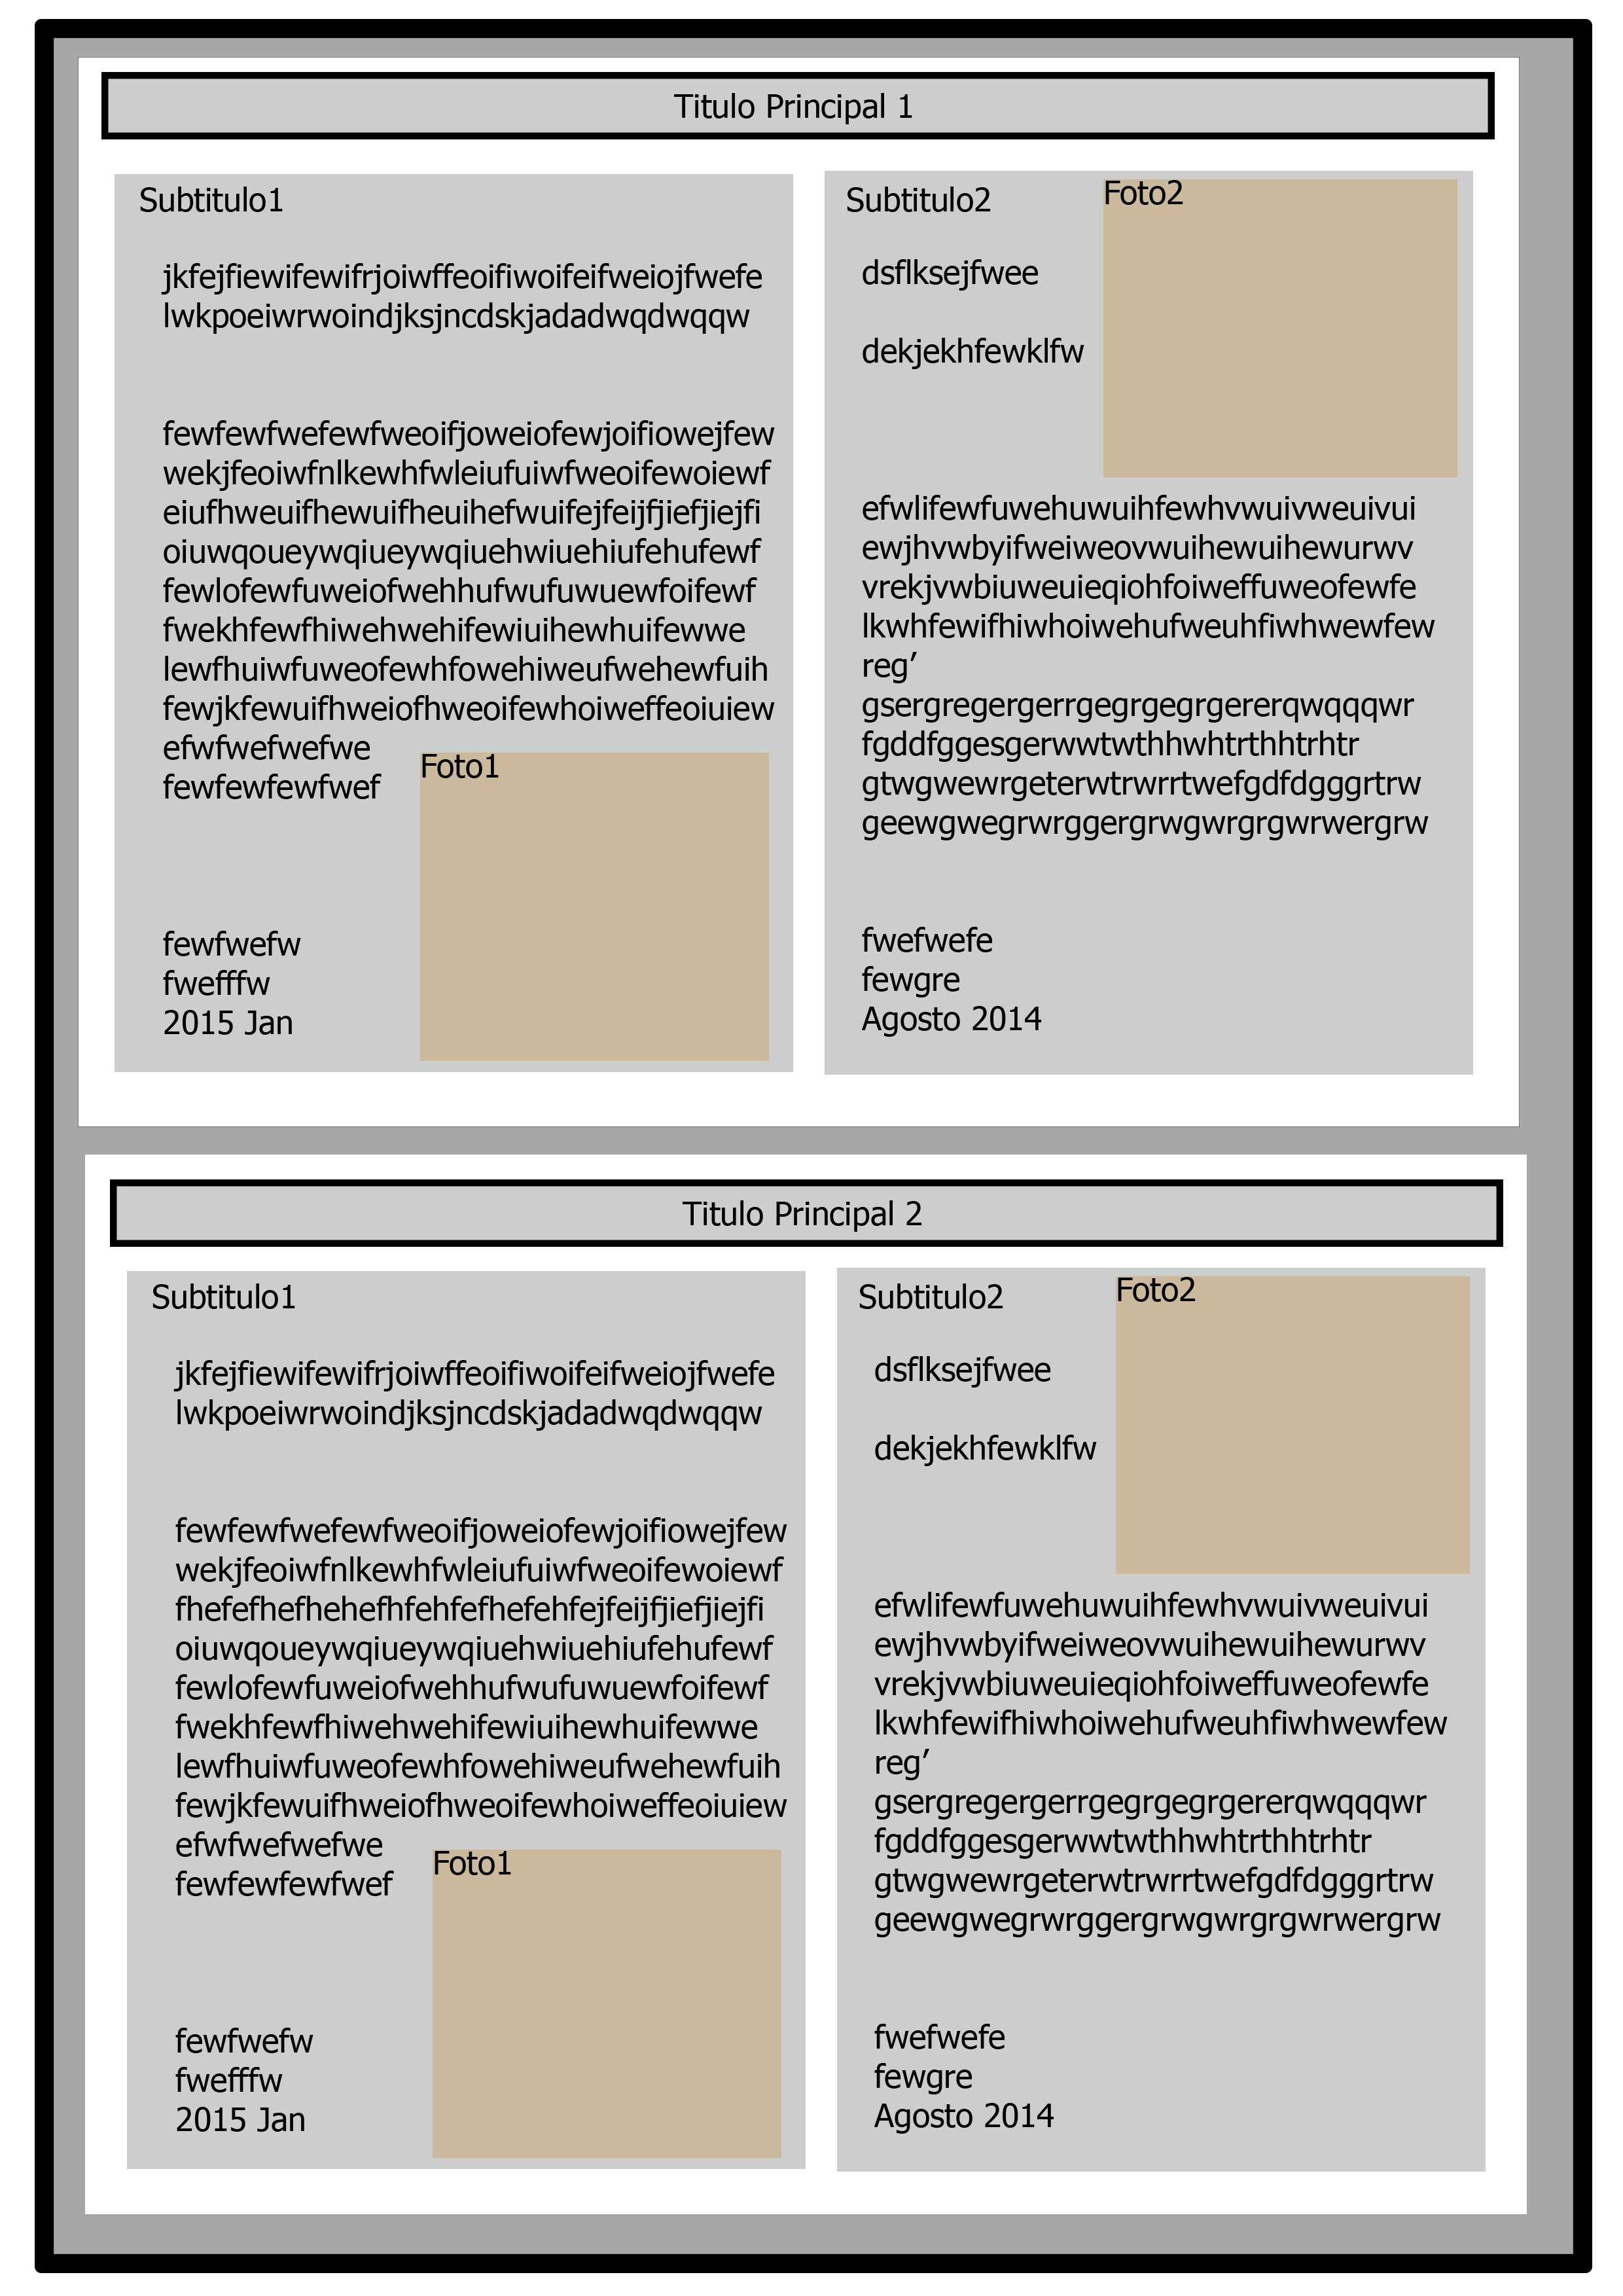
\includegraphics[\linewidth, height=15cm]{layoutnoticias.jpg} 

\caption{Figura 4: Menu de Conteúdo}

\end{document}